\chapter{Technologien}

%
% TypeScript
%
\section{TypeScript}

TypeScript ist eine Programmiersprache von Microsoft, die JavaScript um ein Typensystem erweitert. So können u.A. Fehler frühzeitig (während der Entwicklung) erkannt und behoben sowie Autovervollständigungen geboten werden. TypeScript-Code kann nicht direkt ausgeführt werden, sondern muss vorher zu JavaScript transpiliert werden. Jeder gültige JavaScript-Code ist dadurch auch gültiger TypeScript-Code \cites[vgl.][]{TypeScript}[vgl.][]{TypeScriptForJSDevelopers}.

Codebeispiel \ref{lst:typescript} zeigt einen TypeScript-Code, bei dem der Parameter der Funktion als Array typisiert wurde. Wird nun z.B. eine ungültige Methode, wie \lstinline{trim} aufgerufen, gibt TypeScript eine Fehlermeldung aus, da Arrays diese Methode nicht besitzen.

\vspace{2\parskip}
\begin{minipage}{\linewidth}
  \begin{lstlisting}[language=java, frame=single, label=lst:typescript, caption=Beispiel für TypeScript-Code]
    function compact(arr: any[]) {
      if (arr.length > 0)
        // Error: Property 'trim' does not exist on type 'any[]'.
        return arr.trim(0, 10);
      return arr;
    }
  \end{lstlisting}
\end{minipage}

Bestehende JavaScript-Projekte können inkrementell auf TypeScript umgestellt werden, indem TypeScript vorerst nur als Typ-Überprüfung verwendet wird. Dabei können Kommentare in den vorhandenen JavaScript-Code eingefügt werden, wodurch TypeScript anschließend den Code überprüfen kann (siehe Codebeispiel \ref{lst:typescript-inkrementell}) \cite[vgl.][]{TypeScript}. Da hierbei anders als in Codebeispiel \ref{lst:typescript} kein TypeScript-Code eingefügt wird, muss der Code nicht transpiliert werden, bietet jedoch auch nicht den vollen Funktionsumfang von TypeScript.

\begin{minipage}{\linewidth}
  \begin{lstlisting}[language=java, frame=single, label=lst:typescript-inkrementell, caption=Erweiterung von JavaScript-Code um TypeScript Typ-Überprüfung]
    // @ts-check

    /** @param {any[]} arr */
    function compact(arr) {
      if (arr.length > 0)
        // Error: Property 'trim' does not exist on type 'any[]'.
        return arr.trim(0, 10);
      return arr;
    }
  \end{lstlisting}
\end{minipage}

%
% Vue.js
%
\section{Vue}

Für die Erstellung der Benutzeroberfläche (im Folgenden \glqq Frontend\grqq{} genannt) wird Vue verwendet. Vue ist ein progressives JavaScript-Framework, das die Frontend-Entwicklung vereinfachen soll. Progressiv bedeutet hierbei, das es für das gesamte Frontend oder auch nur für Teile dessen verwendet werden kann. Vue kann folglich mit anderen Technologien verwendet oder Schritt-für-Schritt (progressiv) in bereits vorhandene Projekte integriert werden \cite[vgl.][]{VueIntroduction}.

\subsection{Komponenten}
\begin{figure}[H]
  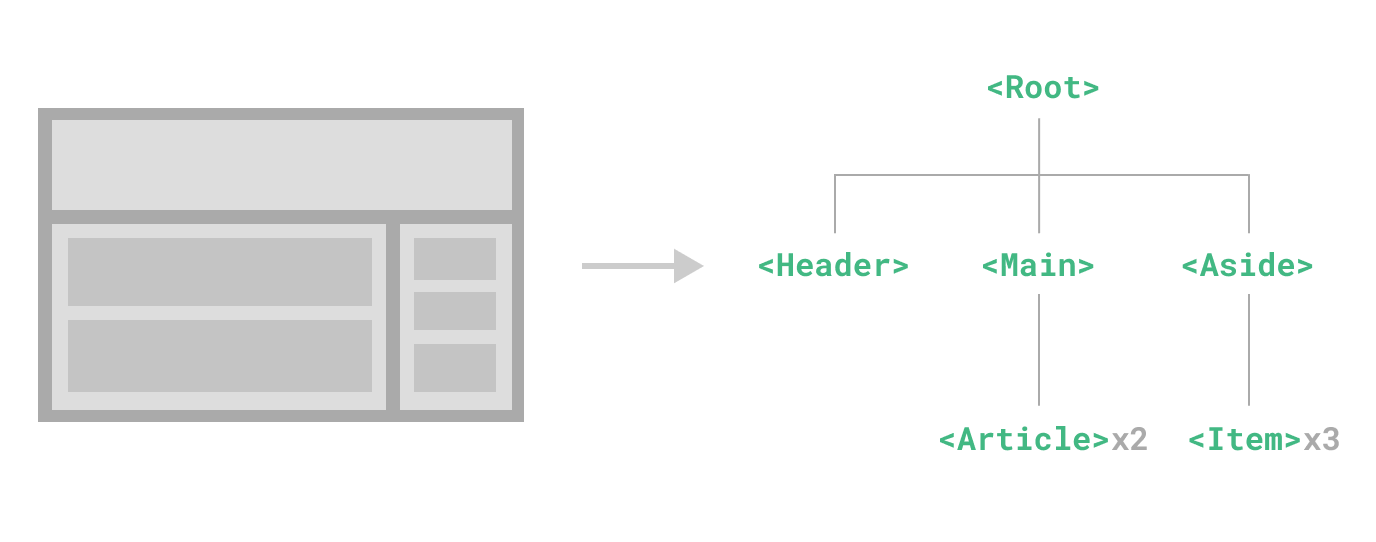
\includegraphics[width=0.8\textwidth]{images/vue-components.png}
  \centering
  \caption[Vue-Komponenten]{Strukturierung des Frontends durch Vue-Komponenten \cite{VueComponentBasics}}
  \label{fig:vue-components}
\end{figure}

Vue-Komponenten erlauben die Unterteilung des Frontends in unabhängige, isolierte und wiederverwendbare Teile. So wird das Frontend in kleinere Komponenten gegliedert (siehe Abbildung \ref{fig:vue-components}), die dann die benötigte Logik kapseln und unabhängig entwickelt werden können \cite[vgl.][]{VueComponentBasics}.

Vue bietet mehrere Möglichkeiten, um eine Komponente zu definieren. Im Rahmen dieser Studienarbeit werden sogenannte \aclu{SFC} (\acs{SFC}) verwendet. Jede Komponente wird hierbei in einer Datei mit der Dateiendung \lstinline{.vue} definiert \cite[vgl.][]{VueComponentBasics}.

\vspace{2\parskip}
\begin{minipage}{\linewidth}
  \begin{lstlisting}[language=java, frame=single, label=lst:vue-component, caption=Beispiel einer Vue \ac{SFC}]
    <script setup>
    import { ref } from 'vue'

    const count = ref(0)
    </script>

    <template>
      <button @click="count++">You clicked me {{ count }} times.</button>
    </template>
  \end{lstlisting}
\end{minipage}

%
% Strapi CMS
%
\section{Strapi CMS}

%
% Heroku
%
\section{Heroku}
